\documentclass[12pt,a4paper]{report}
\usepackage{tikz}
\usepackage{geometry}

\usetikzlibrary{external, shapes.geometric, arrows, arrows.meta}

\tikzexternalize[prefix=tikz/] % Externalize TikZ figures and store them in the "tikz/" folder

\tikzset{
    svg export/.style={
        % Configure for SVG export
        external/system call/.add={}{; pdftocairo -svg "\image.pdf" "\image.svg"},
        % Use the SVG figure instead of the PDF
        /pgf/images/external info,
        /pgf/images/include external/.code={%
            \includegraphics[width=\pgfexternalwidth,height=\pgfexternalheight]{##1.svg}
        },
    }
}

\begin{document}
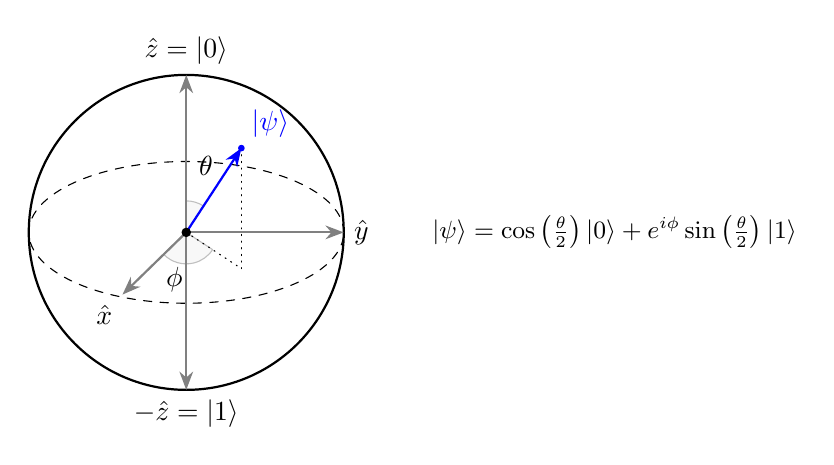
\begin{tikzpicture}[line cap=round, line join=round, >=Stealth]
            
    % Draw the outer sphere
    \draw[thick] (0,0) circle (2cm);
    
    % Draw the equatorial plane (dashed ellipse)
    \draw[dash pattern=on 3pt off 3pt] (0,0) ellipse (2cm and 0.9cm);
    
    % Highlight angles
    \draw[shift={(0,0)}, lightgray, fill, fill opacity=0.1] (0,0) -- (56.7:0.4) arc (56.7:90:0.4) -- cycle;
    \draw[shift={(0,0)}, lightgray, fill, fill opacity=0.1] (0,0) -- (-135.7:0.4) arc (-135.7:-33.2:0.4) -- cycle;
    
    % Axes
    \draw[->, thick, gray] (0,0) -- (0,2) node[anchor=south, black] {$\hat{z}=|0\rangle$};
    \draw[->, thick, gray] (0,0) -- (2,0) node[anchor=west, black] {$\hat{y}$};
    \draw[->, thick, gray] (0,0) -- (-0.81,-0.79) node[anchor=north east, black] {$\hat{x}$};
    \draw[->, thick, gray] (0,0) -- (0,-2) node[anchor=north, black] {$-\hat{z}=|1\rangle$};
    
    % Qubit state vector
    \draw[thick, ->, blue] (0,0) -- (0.7,1.07) node[anchor=south west] {$|\psi\rangle$};
    
    % Projection lines
    \draw[dotted] (0.7,1.07) -- (0.7,-0.46);
    \draw[dotted] (0,0) -- (0.7,-0.46);
    
    % Angle labels
    \node at (-0.15,-0.6) {$\phi$};
    \node at (0.25,0.85) {$\theta$}; % Adjusted theta position slightly to the right
    
    % State label moved to the side
    \node[align=left, font=\small, anchor=west] at (3,0) {$|\psi\rangle = \cos\left(\frac{\theta}{2}\right)|0\rangle + e^{i\phi}\sin\left(\frac{\theta}{2}\right)|1\rangle$};
    
    % Markers
    \draw[fill] (0,0) circle (1.5pt); % Origin
    \draw[fill, blue] (0.7,1.07) circle (1pt); % Qubit state
\end{tikzpicture}
\end{document}
